% Provenance (never printed): cycle 3 "La planete Terre" (natural phenomena
% and the risks they bring: storms, floods, droughts, earthquakes, eruptions;
% warnings and the right behaviour); see sources/book1/PROVENANCE.md.
% Book 1, grade 5, chapter 3.
\chapter{Bahaya Alam}\label{ch:g5:natural-hazards}

Hari Jumat malam. Di radio, musik berhenti dan sebuah suara yang tenang
membacakan peringatan: \omterm{def:g5:natural-hazards:storm}{badai} yang kuat akan mencapai \omterm{def:g1:landscapes-around-us:water}{pesisir} malam ini,
dengan angin yang sangat kencang dan \omterm{def:g4:clouds-rain-snow:precipitation}{hujan} lebat. Semua orang diminta tetap
di dalam rumah mulai pukul sembilan dan mengikat atau memasukkan segala
sesuatu yang dapat diterbangkan angin.

Keluarga Lena mulai bekerja. Ayahnya memasukkan kursi dan meja taman ke
dalam gudang. Ibunya memeriksa apakah senter-senter menyala dan menaruh
baterai cadangan di meja dapur. Lena mengisi dua botol besar dengan air.
Pada pukul sembilan, semua orang sudah berada di dalam, dan angin sudah
menderu-deru.

\begin{omfigure}
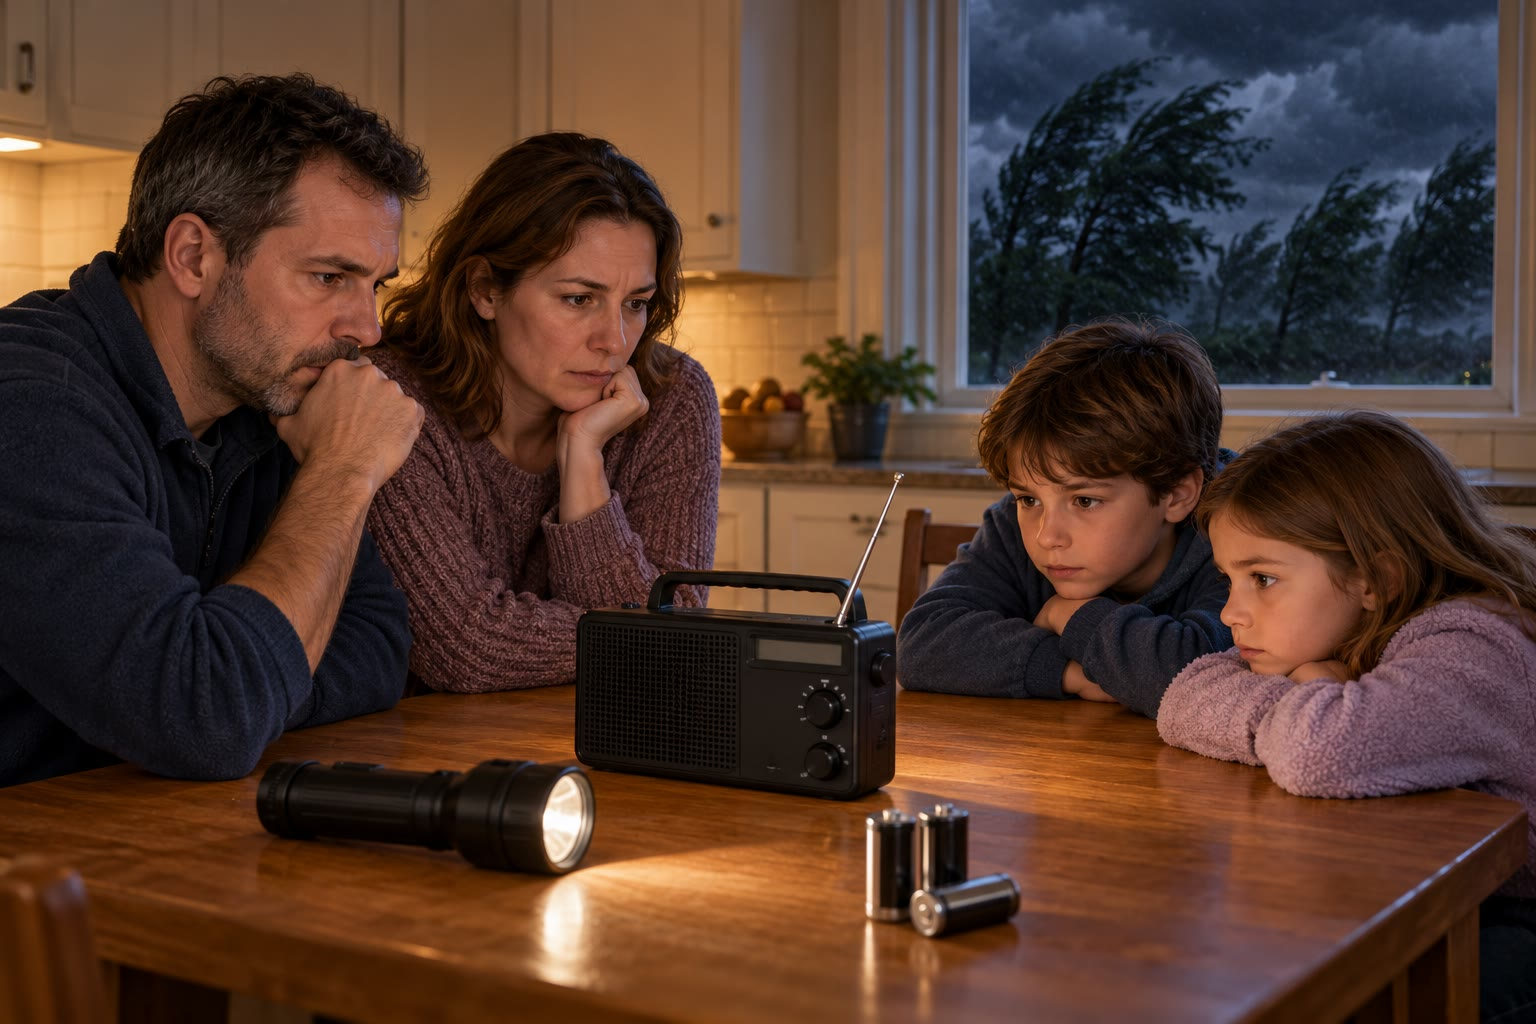
\includegraphics[width=0.5\linewidth]{images/book1/ai/g5-radio-warning.jpg}

{\small Sebuah keluarga mendengarkan peringatan \omterm{def:g5:natural-hazards:storm}{badai} di radio, dengan senter
dan baterai cadangan yang sudah siap.}
\end{omfigure}

\begin{recall}
\omterm{def:g4:volcanoes-earthquakes-first-look:volcano}{Gunung api} dapat meletus, menyemburkan \omterm{def:g4:volcanoes-earthquakes-first-look:eruption}{lava}, abu, dan gas; \omterm{def:g4:volcanoes-earthquakes-first-look:earthquake}{gempa bumi} adalah
guncangan tanah yang tiba-tiba; ketika \omterm{def:g4:volcanoes-earthquakes-first-look:earthquake}{gempa bumi}, kita merunduk,
berlindung, dan berpegangan (\cref{ch:g4:volcanoes-earthquakes-first-look}).
\omterm{def:g1:landscapes-around-us:water}{Sungai} yang menerima lebih banyak air daripada yang dapat ditampung alurnya
akan membanjiri \omterm{def:g5:water-shapes-the-land:flood}{dataran banjirnya} (\cref{ch:g5:water-shapes-the-land}).
Setiap tempat mempunyai \omterm{def:g5:weather-and-climate:climate}{iklimnya} sendiri, dan zona panas, zona sedang, dan
zona dingin melingkari \omterm{def:g3:continents-and-oceans:globe}{bola dunia} (\cref{ch:g5:weather-and-climate}).
\end{recall}

\section{Apa itu bahaya alam}

Alam tidak selalu tenang. Angin dapat bertiup cukup kencang untuk
mematahkan pohon, \omterm{def:g1:landscapes-around-us:water}{sungai} dapat \omterm{def:g5:water-shapes-the-land:flood}{banjir}, tanah dapat berguncang. Peristiwa
seperti ini adalah bagian dari cara kerja Bumi: semuanya sudah terjadi jauh
sebelum ada manusia, dan akan terus terjadi.

\begin{definition}[Bahaya alam]\label{def:g5:natural-hazards:hazard}
Yang disebut \emph{bahaya alam}\index{bahaya alam} adalah peristiwa alam yang
dapat mencelakai manusia atau merusak apa yang telah mereka bangun: \omterm{def:g5:natural-hazards:storm}{badai},
\omterm{def:g5:water-shapes-the-land:flood}{banjir}, \omterm{def:g5:natural-hazards:drought}{kekeringan}, \omterm{def:g4:volcanoes-earthquakes-first-look:earthquake}{gempa bumi}, \omterm{def:g4:volcanoes-earthquakes-first-look:eruption}{letusan} \omterm{def:g4:volcanoes-earthquakes-first-look:volcano}{gunung api}, \omterm{def:g5:natural-hazards:landslide}{tanah longsor}{\ldots}
\end{definition}

Kita dapat mengelompokkan \omterm{def:g5:natural-hazards:hazard}{bahaya alam} menurut asalnya: dari udara, dari
air, atau dari tanah.

\begin{omfigure}
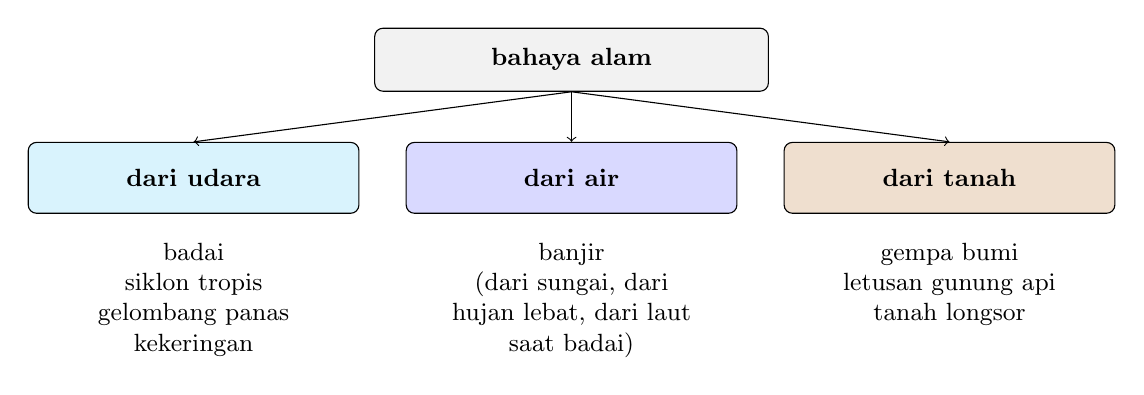
\begin{tikzpicture}[font=\small, box/.style={draw, rounded corners=3pt,
    minimum width=4.2cm, minimum height=0.9cm, align=center}]
  \node[box, fill=cyan!15, font=\small\bfseries] (A) at (0,0) {dari udara};
  \node[box, fill=blue!15, font=\small\bfseries] (W) at (4.8,0) {dari air};
  \node[box, fill=brown!25, font=\small\bfseries] (G) at (9.6,0) {dari tanah};
  \node[align=center, anchor=north] at (0,-0.7) {badai\\siklon tropis\\gelombang panas\\kekeringan};
  \node[align=center, anchor=north] at (4.8,-0.7) {banjir\\(dari sungai, dari\\hujan lebat, dari laut\\saat badai)};
  \node[align=center, anchor=north] at (9.6,-0.7) {gempa bumi\\letusan gunung api\\tanah longsor};
  \node[draw, rounded corners=3pt, fill=gray!10, font=\small\bfseries,
    minimum width=5cm, minimum height=0.8cm] (N) at (4.8,1.5) {bahaya alam};
  \draw[->] (N.south) -- (A.north);
  \draw[->] (N.south) -- (W.north);
  \draw[->] (N.south) -- (G.north);
\end{tikzpicture}

{\small \omterm{def:g5:natural-hazards:hazard}{Bahaya alam}, dikelompokkan menurut asalnya.}
\end{omfigure}

\section{Bahaya dari udara}

\begin{definition}[Badai]\label{def:g5:natural-hazards:storm}
Yang disebut \emph{badai}\index{badai} adalah masa ketika angin bertiup
sangat kencang, biasanya disertai \omterm{def:g4:clouds-rain-snow:precipitation}{hujan} lebat atau \omterm{def:g4:clouds-rain-snow:precipitation}{salju}, dan kadang-kadang
disertai guruh dan kilat.
\end{definition}

\omterm{def:g5:natural-hazards:storm}{Badai} yang kuat mematahkan dahan, menumbangkan pohon, menerbangkan genting
dari atap, dan dapat melemparkan kursi taman menembus jendela. Di \omterm{def:g1:landscapes-around-us:water}{pesisir},
anginnya menumpuk air \omterm{def:g2:water-on-earth:ocean}{laut} ke arah pantai dan mengirimkan ombak raksasa
melewati tembok \omterm{def:g2:water-on-earth:ocean}{laut}.

\omterm{def:g5:natural-hazards:storm}{Badai} yang paling dahsyat di Bumi terbentuk di atas \omterm{def:g2:water-on-earth:ocean}{laut} tropis yang
hangat. \omterm{def:g5:natural-hazards:storm}{Badai} ini sangat besar dan berputar: dari antariksa, \omterm{def:g5:natural-hazards:storm}{badai} ini
tampak seperti spiral \omterm{def:g4:clouds-rain-snow:cloud}{awan} raksasa, dengan lubang yang tenang dan cerah di
tengahnya, yaitu mata \omterm{def:g5:natural-hazards:storm}{badai}. Di sekeliling mata \omterm{def:g5:natural-hazards:storm}{badai} bertiup angin yang
paling kencang. \omterm{def:g5:natural-hazards:storm}{Badai} yang sama jenisnya mempunyai nama yang berbeda di
\omterm{def:g2:water-on-earth:ocean}{samudra} yang berbeda: \omterm{def:g5:natural-hazards:storm}{badai} ini disebut \emph{hurikan} di Atlantik Utara
dan di Pasifik timur, \emph{taifun} di Pasifik barat laut, dan
\emph{siklon tropis} di Pasifik Selatan dan \omterm{def:g2:water-on-earth:ocean}{Samudra} Hindia.
% ledger: noaa:cyclone-names

\begin{omfigure}
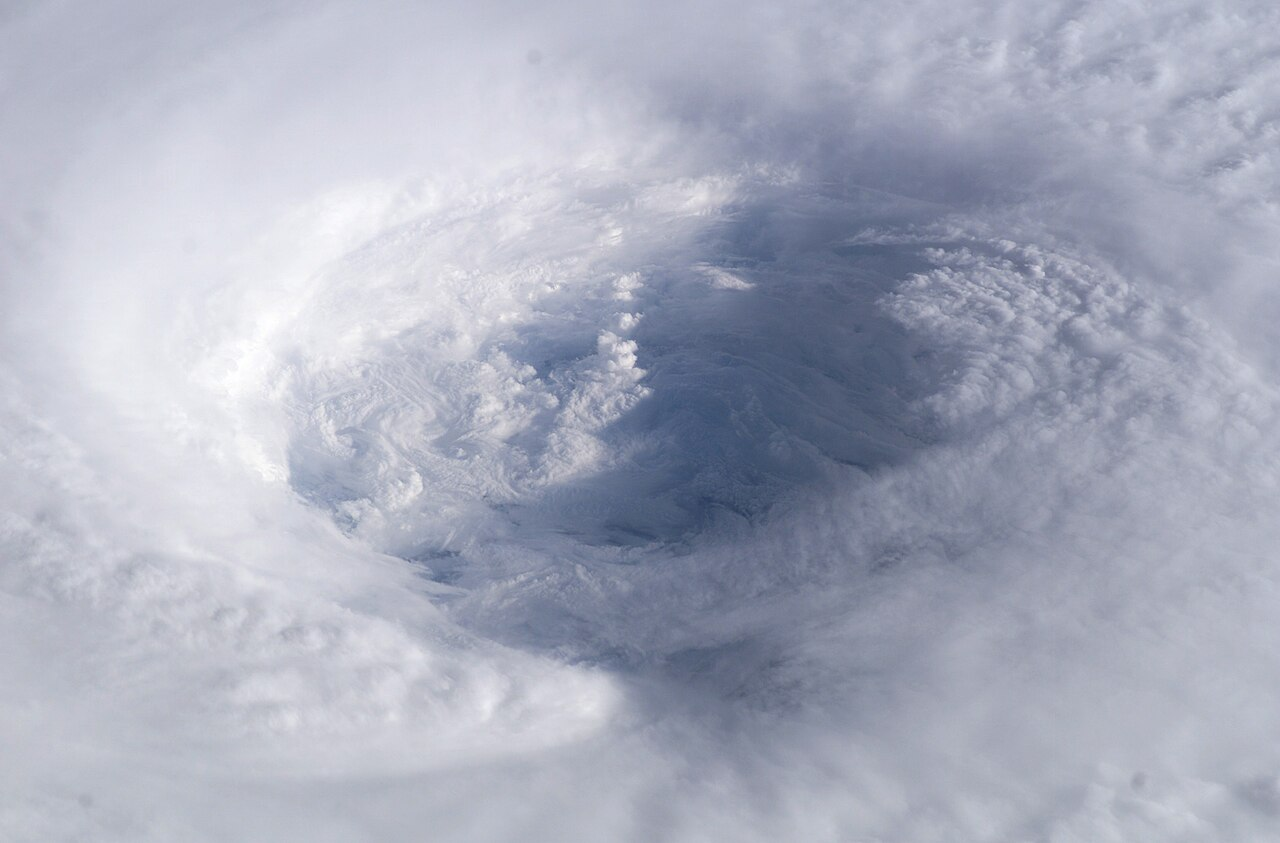
\includegraphics[width=0.5\linewidth]{images/book1/g5-hurricane-isabel-iss.jpg}

{\small Memandang ke bawah, ke mata Hurikan Isabel, di atas \omterm{def:g2:water-on-earth:ocean}{Samudra}
Atlantik pada bulan September 2003, dari Stasiun Antariksa Internasional:
dinding \omterm{def:g4:clouds-rain-snow:cloud}{awan} di sekeliling pusat yang lebih tenang. Foto: NASA (domain
publik).}
% ledger: nasa:isabel-iss
\end{omfigure}

Sebagian bahaya dari udara datang dengan lambat dan diam-diam.
\emph{Gelombang panas} adalah masa beberapa hari dan malam yang jauh lebih
panas daripada biasanya. Gelombang panas berbahaya terutama bagi orang
yang sangat tua, bayi, dan orang sakit.

\begin{definition}[Kekeringan]\label{def:g5:natural-hazards:drought}
Yang disebut \emph{kekeringan}\index{kekeringan} adalah masa yang panjang,
berbulan-bulan atau bahkan bertahun-tahun, dengan \omterm{def:g4:clouds-rain-snow:precipitation}{hujan} yang jauh lebih
sedikit daripada biasanya di tempat itu. Tanah mengering, \omterm{def:g1:landscapes-around-us:water}{sungai} dan \omterm{def:g1:landscapes-around-us:water}{danau}
menyusut, tanaman layu dan mati.
\end{definition}

\omterm{def:g5:natural-hazards:drought}{Kekeringan} datang perlahan-lahan: tidak ada yang dapat mengatakan pada hari
apa \omterm{def:g5:natural-hazards:drought}{kekeringan} itu mulai. Akan tetapi, \omterm{def:g5:natural-hazards:drought}{kekeringan} yang panjang dapat membuat
petani tidak panen dan kota-kota kekurangan air.

\begin{omfigure}
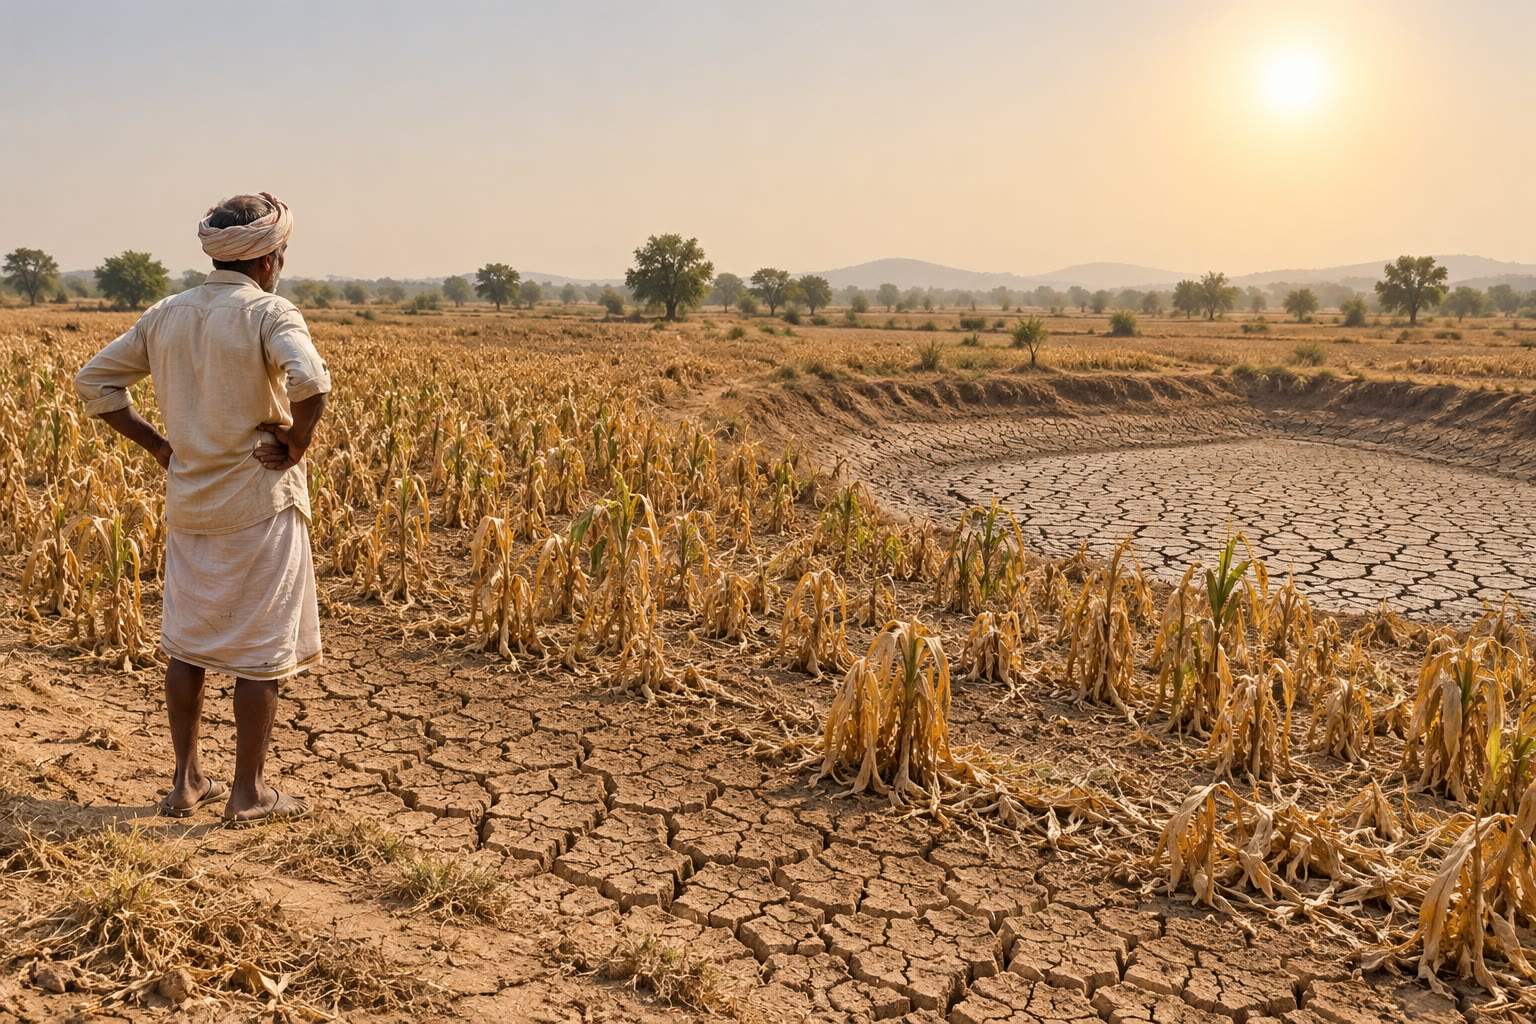
\includegraphics[width=0.42\linewidth]{images/book1/ai/g5-drought-field.jpg}

{\small Sebidang ladang dalam \omterm{def:g5:natural-hazards:drought}{kekeringan} yang panjang: tanahnya retak-retak,
tanamannya menguning, dan kolamnya sudah kering.}
\end{omfigure}

\section{Bahaya dari air}

Kamu sudah mengenal \omterm{def:g5:water-shapes-the-land:flood}{banjir} \omterm{def:g1:landscapes-around-us:water}{sungai} (\cref{ch:g5:water-shapes-the-land}).
Setelah berhari-hari \omterm{def:g4:clouds-rain-snow:precipitation}{hujan}, atau ketika \omterm{def:g4:clouds-rain-snow:precipitation}{salju} mencair dengan cepat, \omterm{def:g1:landscapes-around-us:water}{sungai}
naik melewati tepinya dan menggenangi \omterm{def:g5:water-shapes-the-land:flood}{dataran banjirnya}. Ada \omterm{def:g5:water-shapes-the-land:flood}{banjir} yang
datang sangat cepat: \omterm{def:g4:clouds-rain-snow:precipitation}{hujan} deras yang hebat di \omterm{def:g1:landscapes-around-us:landform}{lembah} yang curam dapat
mengubah \omterm{def:g1:landscapes-around-us:water}{sungai} kecil yang tenang menjadi arus deras yang menderu dalam
waktu satu jam. Ada pula \omterm{def:g5:water-shapes-the-land:flood}{banjir} yang datang dari \omterm{def:g2:water-on-earth:ocean}{laut}, ketika \omterm{def:g5:natural-hazards:storm}{badai}
mendorong air naik ke \omterm{def:g1:landscapes-around-us:water}{pesisir} yang rendah.

\section{Bahaya dari tanah}

Kamu sudah mengenal \omterm{def:g4:volcanoes-earthquakes-first-look:earthquake}{gempa bumi} dan \omterm{def:g4:volcanoes-earthquakes-first-look:eruption}{letusan} \omterm{def:g4:volcanoes-earthquakes-first-look:volcano}{gunung api}
(\cref{ch:g4:volcanoes-earthquakes-first-look}). Ada bahaya ketiga yang
datang dari tanah, dan air sering kali memicunya.

\begin{definition}[Tanah longsor]\label{def:g5:natural-hazards:landslide}
Yang disebut \emph{tanah longsor}\index{tanah longsor} adalah massa \omterm{def:g3:stones-pebbles-sand:rock}{batuan},
tanah, atau \omterm{def:g3:stones-pebbles-sand:sand}{lumpur} yang tiba-tiba meluncur atau runtuh menuruni lereng.
\end{definition}

Lereng curam yang basah kuyup oleh \omterm{def:g4:clouds-rain-snow:precipitation}{hujan} yang panjang menjadi berat dan
licin, dan lereng itu dapat runtuh sekaligus. \omterm{def:g4:volcanoes-earthquakes-first-look:earthquake}{Gempa bumi} juga dapat
mengguncang lereng sampai lepas. \omterm{def:g5:natural-hazards:landslide}{Tanah longsor} dapat mengubur jalan,
membendung \omterm{def:g1:landscapes-around-us:water}{sungai}, atau menghanyutkan rumah.

\begin{omfigure}
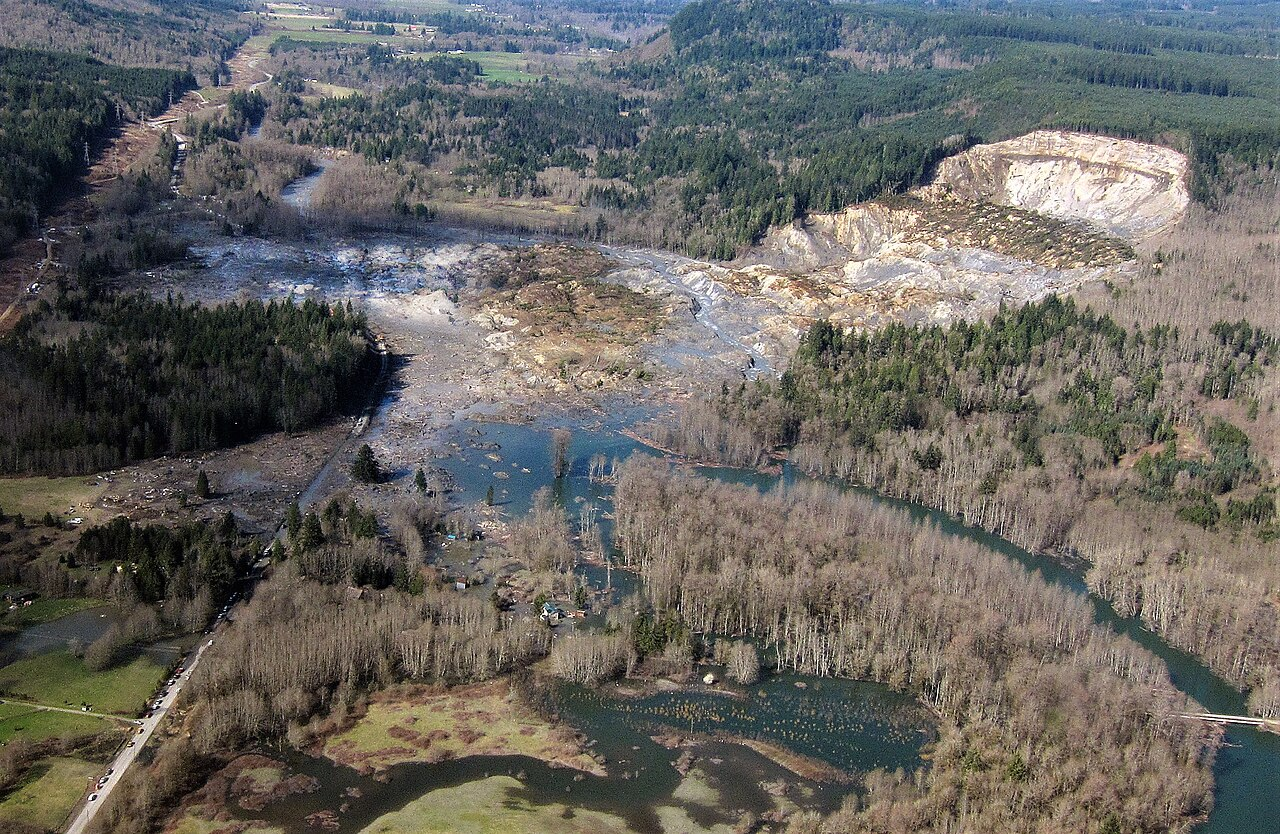
\includegraphics[width=0.6\linewidth]{images/book1/g5-landslide-washington.jpg}

{\small \omterm{def:g5:natural-hazards:landslide}{Tanah longsor} besar di Negara Bagian Washington, di Amerika Serikat,
pada tahun 2014, dilihat dari pesawat. Lereng \omterm{def:g1:landscapes-around-us:landform}{bukit} di sebelah kanan telah
runtuh; \omterm{def:g3:stones-pebbles-sand:sand}{lumpurnya} menyebar ke seluruh \omterm{def:g1:landscapes-around-us:landform}{lembah}, menutupi jalan, dan
membendung \omterm{def:g1:landscapes-around-us:water}{sungai}, yang lalu menggenangi hutan di hulu. Foto: Mark Reid,
U.S. Geological Survey (domain publik).}\label{fig:g5:natural-hazards:landslide}
% ledger: usgs:oso-aerial
\end{omfigure}

\section{Dari bahaya menjadi bencana}

\omterm{def:g5:natural-hazards:storm}{Badai} di tengah \omterm{def:g2:water-on-earth:ocean}{samudra}, \omterm{def:g4:volcanoes-earthquakes-first-look:earthquake}{gempa bumi} di \omterm{def:g5:weather-and-climate:desert}{gurun} yang kosong, \omterm{def:g5:water-shapes-the-land:flood}{banjir} di \omterm{def:g1:landscapes-around-us:landform}{lembah}
yang tidak berpenghuni: semua itu adalah \omterm{def:g5:natural-hazards:hazard}{bahaya alam}, tetapi tidak
mencelakai siapa pun. Peristiwa yang sama menjadi berbahaya ketika terjadi
di tempat manusia tinggal.

\begin{definition}[Bencana alam]\label{def:g5:natural-hazards:disaster}
Yang disebut \emph{bencana alam}\index{bencana alam} terjadi ketika \omterm{def:g5:natural-hazards:hazard}{bahaya
alam} melanda tempat manusia tinggal dan menimbulkan kerugian besar: orang
terluka atau tewas, rumah hancur, jalan, air, dan listrik terputus.
\end{definition}

\begin{omfigure}
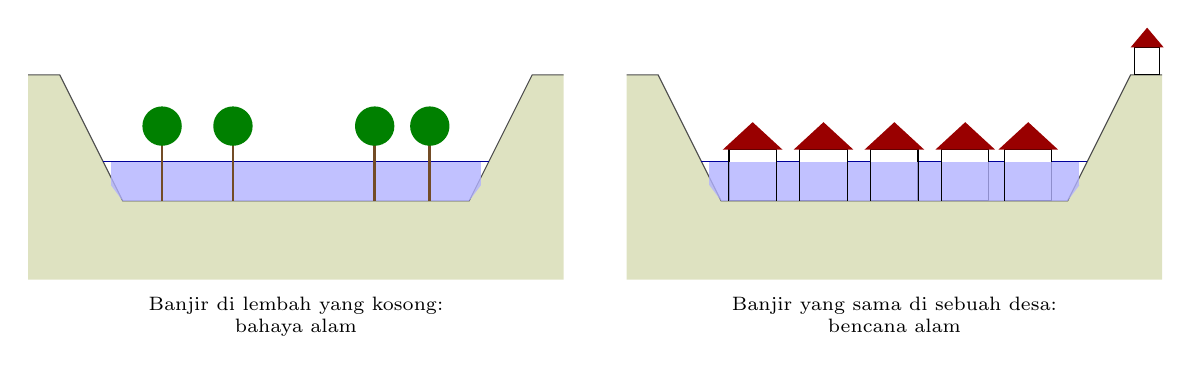
\begin{tikzpicture}[x=1cm, y=1cm, font=\scriptsize]
  \foreach \dx/\title in {0/{Banjir di lembah yang kosong:\\bahaya alam},
                          7.6/{Banjir yang sama di sebuah desa:\\bencana alam}} {
    \begin{scope}[xshift=\dx cm]
      % valley sides
      \fill[green!25!brown!30] (0,0) -- (0,2.6) -- (0.4,2.6) -- (1.2,1.0) -- (5.6,1.0)
        -- (6.4,2.6) -- (6.8,2.6) -- (6.8,0) -- cycle;
      \draw[gray!60!black] (0,2.6) -- (0.4,2.6) -- (1.2,1.0) -- (5.6,1.0) -- (6.4,2.6) -- (6.8,2.6);
      % flood water over the whole valley floor
      \fill[blue!30, opacity=0.8] (1.05,1.2) -- (5.75,1.2) -- (5.6,1.0) -- (1.2,1.0) -- cycle;
      \fill[blue!30, opacity=0.8] (1.05,1.2) rectangle (5.75,1.5);
      \draw[blue!60!black] (0.95,1.5) -- (5.85,1.5);
      \node[align=center, anchor=north] at (3.4,-0.1) {\title};
    \end{scope}
  }
  % trees in the empty valley
  \foreach \x in {1.7,2.6,4.4,5.1} {
    \draw[brown!60!black, line width=1pt] (\x,1.0) -- (\x,1.75);
    \fill[green!50!black] (\x,1.95) circle (0.25);
  }
  % houses in the village valley
  \begin{scope}[xshift=7.6cm]
    \foreach \x in {1.6,2.5,3.4,4.3,5.1} {
      \fill[white, draw=black] (\x-0.3,1.0) rectangle (\x+0.3,1.65);
      \fill[red!60!black] (\x-0.38,1.65) -- (\x,2.0) -- (\x+0.38,1.65) -- cycle;
      \fill[blue!30, opacity=0.8] (\x-0.3,1.0) rectangle (\x+0.3,1.5);
    }
    % one house on the high ground, dry
    \fill[white, draw=black] (6.45,2.6) rectangle (6.77,2.95);
    \fill[red!60!black] (6.40,2.95) -- (6.61,3.2) -- (6.82,2.95) -- cycle;
  \end{scope}
\end{tikzpicture}

{\small \omterm{def:g5:water-shapes-the-land:flood}{Banjir} yang sama, dua kali. Di \omterm{def:g1:landscapes-around-us:landform}{lembah} yang kosong, \omterm{def:g5:water-shapes-the-land:flood}{banjir} itu tidak
mencelakai siapa pun; di tempat sebuah desa dibangun di \omterm{def:g5:water-shapes-the-land:flood}{dataran banjir},
\omterm{def:g5:water-shapes-the-land:flood}{banjir} itu menggenangi rumah-rumah. Rumah di tanah yang tinggi tetap
kering.}
\end{omfigure}

Kita tidak dapat menghentikan \omterm{def:g5:natural-hazards:storm}{badai} atau \omterm{def:g4:volcanoes-earthquakes-first-look:earthquake}{gempa bumi}. Akan tetapi, banyak
yang dapat kita lakukan agar bahaya tidak berubah menjadi bencana:
membangun jauh dari \omterm{def:g5:water-shapes-the-land:flood}{dataran banjir} dan dari kaki lereng yang tidak stabil,
membuat bangunan yang kuat, mengamati \omterm{def:g1:watching-the-weather:weather}{cuaca} dan tanah, memperingatkan
orang tepat waktu, dan mengajari semua orang apa yang harus dilakukan.

\subsection*{Peringatan}

Badan \omterm{def:g1:watching-the-weather:weather}{cuaca} mengamati langit siang dan malam. Ketika \omterm{def:g5:natural-hazards:storm}{badai}, gelombang
panas, atau \omterm{def:g5:water-shapes-the-land:flood}{banjir} akan datang, mereka mengirimkan peringatan melalui
radio, televisi, telepon, dan internet. Banyak negara memakai warna, dari
yang paling tenang sampai yang paling serius.

\begin{omfigure}
\begin{tikzpicture}[font=\small, wstep/.style={draw=black!60, minimum width=2.6cm,
    minimum height=0.8cm, font=\small\bfseries, rounded corners=2pt}]
  \node[wstep, fill=green!45] (g) at (0,0) {hijau};
  \node[wstep, fill=yellow!60] (y) at (0.6,0.95) {kuning};
  \node[wstep, fill=orange!70] (o) at (1.2,1.9) {oranye};
  \node[wstep, fill=red!65, text=white] (r) at (1.8,2.85) {merah};
  \node[anchor=west] at ($(g.east)+(0.3,0)$) {tidak ada bahaya khusus};
  \node[anchor=west] at ($(y.east)+(0.3,0)$) {berhati-hatilah, ikuti terus kabarnya};
  \node[anchor=west] at ($(o.east)+(0.3,0)$) {bersiaplah: bahaya mungkin terjadi};
  \node[anchor=west] at ($(r.east)+(0.3,0)$) {bahaya besar: bertindaklah sekarang, ikuti petunjuk};
\end{tikzpicture}

{\small Tangga warna peringatan. Arti tepatnya berbeda dari satu negara ke
negara lain: selalu dengarkan petunjuk yang diberikan bersama peringatan
itu.}
\end{omfigure}

\begin{safety}
\textbf{Saat \omterm{def:g5:natural-hazards:storm}{badai}.} Tetaplah di dalam rumah, jauh dari jendela. Jangan
keluar untuk melihat-lihat, dan jauhilah pohon, yang dapat tumbang, serta
kabel listrik yang putus.

\textbf{Saat \omterm{def:g5:water-shapes-the-land:flood}{banjir}.} Pindahlah ke tanah yang lebih tinggi atau ke lantai
atas. Jangan pernah berjalan, bersepeda, atau naik mobil melewati air
\omterm{def:g5:water-shapes-the-land:flood}{banjir}: sedikit air yang deras sudah cukup untuk menjatuhkanmu atau
menghanyutkan mobil.

\textbf{Saat gelombang panas.} Seringlah minum air, tetaplah di tempat teduh
atau di ruangan yang sejuk pada jam-jam yang paling panas, dan tengoklah
tetangga yang sudah lanjut usia.

\textbf{Saat \omterm{def:g4:volcanoes-earthquakes-first-look:earthquake}{gempa bumi}.} Merunduk, berlindung, berpegangan
(\cref{ch:g4:volcanoes-earthquakes-first-look}).

\textbf{Selalu.} Dengarkan peringatan dan segera lakukan apa yang
dikatakan oleh orang yang bertanggung jawab.
\end{safety}

\section{Latihan}

\begin{exercise}[$\star$]\label{exo:g5:natural-hazards:1}
Hanya \omterm{def:g5:natural-hazards:hazard}{bahaya alam}, atau \omterm{def:g5:natural-hazards:disaster}{bencana alam}?
\begin{enumerate}
  \item[(a)] \omterm{def:g4:volcanoes-earthquakes-first-look:earthquake}{Gempa bumi} mengguncang \omterm{def:g5:weather-and-climate:desert}{gurun} yang kosong.
  \item[(b)] \omterm{def:g5:natural-hazards:storm}{Badai} menerbangkan atap banyak rumah di sebuah kota.
  \item[(c)] \omterm{def:g5:natural-hazards:landslide}{Tanah longsor} jatuh ke \omterm{def:g1:landscapes-around-us:landform}{lembah} \omterm{def:g1:landscapes-around-us:landform}{gunung} yang tidak berpenghuni.
  \item[(d)] \omterm{def:g1:landscapes-around-us:water}{Sungai} membanjiri sebuah desa dan menggenangi rumah-rumahnya.
\end{enumerate}
\end{exercise}

\begin{exercise}[$\star$]\label{exo:g5:natural-hazards:2}
Kelompokkan bahaya-bahaya berikut ke dalam tiga keluarga (dari udara, dari
air, dari tanah): \omterm{def:g5:natural-hazards:landslide}{tanah longsor}; gelombang panas; \omterm{def:g5:water-shapes-the-land:flood}{banjir}; \omterm{def:g4:volcanoes-earthquakes-first-look:eruption}{letusan} \omterm{def:g4:volcanoes-earthquakes-first-look:volcano}{gunung
api}; \omterm{def:g5:natural-hazards:storm}{badai}; \omterm{def:g5:natural-hazards:drought}{kekeringan}; \omterm{def:g4:volcanoes-earthquakes-first-look:earthquake}{gempa bumi}.
\end{exercise}

\begin{exercise}[$\star$]\label{exo:g5:natural-hazards:3}
Apa yang dimaksud dengan \omterm{def:g5:natural-hazards:drought}{kekeringan}? Sebutkan dua cara \omterm{def:g5:natural-hazards:drought}{kekeringan} yang panjang mencelakai manusia.
\end{exercise}

\begin{exercise}[$\star$]\label{exo:g5:natural-hazards:4}
Radio mengumumkan peringatan \omterm{def:g5:natural-hazards:storm}{badai} berwarna merah untuk malam ini. Sebutkan
tiga hal yang sebaiknya dilakukan keluargamu.
\end{exercise}

\begin{exercise}[$\star$]\label{exo:g5:natural-hazards:5}
\omterm{def:g5:natural-hazards:storm}{Badai} besar yang berputar dan mempunyai mata terbentuk di atas \omterm{def:g2:water-on-earth:ocean}{laut} tropis
yang hangat. Apa namanya jika \omterm{def:g5:natural-hazards:storm}{badai} itu melanda (a) \omterm{def:g1:landscapes-around-us:water}{pesisir} Florida, di
Atlantik Utara; (b) Jepang, di Pasifik barat laut; (c) \omterm{def:g1:landscapes-around-us:water}{pesisir} India, di
\omterm{def:g2:water-on-earth:ocean}{Samudra} Hindia?
\end{exercise}

\begin{exercise}[$\star$]\label{exo:g5:natural-hazards:6}
Urutkan keempat warna peringatan, dari yang paling tenang sampai yang
paling serius. Apa yang harus kamu lakukan pada tingkat yang paling serius?
\end{exercise}

\begin{exercise}[$\star\star$]\label{exo:g5:natural-hazards:7}
Perhatikan foto \omterm{def:g5:natural-hazards:landslide}{tanah longsor} di
halaman~\pageref{fig:g5:natural-hazards:landslide}. Jelaskan apa yang
dilakukan \omterm{def:g5:natural-hazards:landslide}{tanah longsor} itu terhadap \omterm{def:g1:landscapes-around-us:landform}{lembah}: terhadap lereng \omterm{def:g1:landscapes-around-us:landform}{bukit}, jalan,
dan \omterm{def:g1:landscapes-around-us:water}{sungai}. Mengapa daratan di hulu sekarang tergenang air?
\end{exercise}

\begin{exercise}[$\star\star$]\label{exo:g5:natural-hazards:8}
Tom berkata: ``\omterm{def:g5:water-shapes-the-land:flood}{Banjir} itu alami, jadi tidak ada yang bisa dilakukan.'' Lena
berkata: ``Kita tidak bisa mencegah \omterm{def:g1:landscapes-around-us:water}{sungai} \omterm{def:g5:water-shapes-the-land:flood}{banjir}, tetapi kita bisa mencegah
\omterm{def:g5:water-shapes-the-land:flood}{banjir} menjadi bencana.'' Siapa yang benar? Jelaskan dengan dua contoh.
\end{exercise}

\begin{exercise}[$\star\star$]\label{exo:g5:natural-hazards:9}
Di sebuah daerah pertanian khayalan, biasanya kira-kira 60 milimeter \omterm{def:g4:clouds-rain-snow:precipitation}{hujan}
turun setiap bulan. Selama \omterm{def:g5:natural-hazards:drought}{kekeringan}, hanya seperempat dari \omterm{def:g4:clouds-rain-snow:precipitation}{hujan} yang
biasa turun pada setiap bulan dari empat bulan.
\begin{enumerate}
  \item[(a)] Berapa banyak \omterm{def:g4:clouds-rain-snow:precipitation}{hujan} yang biasanya turun dalam empat bulan?
  \item[(b)] Berapa banyak yang turun selama \omterm{def:g5:natural-hazards:drought}{kekeringan}, dalam empat bulan itu?
  \item[(c)] Berapa banyak \omterm{def:g4:clouds-rain-snow:precipitation}{hujan} yang hilang?
\end{enumerate}
\end{exercise}

\begin{exercise}[$\star\star$]\label{exo:g5:natural-hazards:10}
Sebuah kota khayalan mempunyai 1\,200 rumah. Seperempatnya berdiri di
\omterm{def:g5:water-shapes-the-land:flood}{dataran banjir} \omterm{def:g1:landscapes-around-us:water}{sungainya}.
\begin{enumerate}
  \item[(a)] Berapa banyak rumah yang berdiri di \omterm{def:g5:water-shapes-the-land:flood}{dataran banjir}?
  \item[(b)] Kota itu membantu pemilik sepertiga dari rumah-rumah itu untuk
        pindah ke tanah yang lebih tinggi. Berapa banyak rumah yang masih
        berada di \omterm{def:g5:water-shapes-the-land:flood}{dataran banjir}?
\end{enumerate}
\end{exercise}

\begin{exercise}[$\star\star\star$]\label{exo:g5:natural-hazards:11}
Dua desa yang letaknya berjauhan dilanda \omterm{def:g5:natural-hazards:storm}{badai} dengan kekuatan yang sama
pada malam yang sama. Di desa pertama, tidak ada yang terluka dan
kerusakannya kecil. Di desa kedua, banyak rumah hancur. Berikan
sekurang-kurangnya tiga alasan berbeda yang dapat menjelaskan perbedaan itu.
\end{exercise}
